\phantomsection
\definecolor{dkgreen}{rgb}{0,0.6,0}
\definecolor{gray}{rgb}{0.5,0.5,0.5}
\definecolor{mauve}{rgb}{0.58,0,0.82}


\lstset{frame=tb,
language=R,
aboveskip=3mm,
belowskip=3mm,
showstringspaces=false,
columns=flexible,
numbers=none,
inputencoding=utf8/latin1,
keywordstyle=\color{blue},
numberstyle=\tiny\color{gray},
commentstyle=\color{dkgreen},
stringstyle=\color{mauve},
breaklines=true,
breakatwhitespace=true,
tabsize=3
}


\chapter{Introduzione}\label{cap1}

In ogni età e fase della vita, svolgere attività fisica con regolarità significa fare una scelta a favore della propria salute: praticata regolarmente, l’attività fisica contribuisce a mantenere e migliorare il benessere psicofisico, a ridurre i sintomi di ansia, stress, depressione e solitudine, perché può essere svolta in compagnia, migliora il sonno, aiuta a smettere di fumare. Aiuta la riduzione della pressione arteriosa e il controllo del livello di glicemia e colesterolo nel sangue, aiuta a prevenire malattie metaboliche, cardiovascolari e neoplastiche e artrosi e contribuisce a ridurre il tessuto adiposo in eccesso perché facilita il raggiungimento del bilancio energetico. Comporta benefici evidenti anche per l’apparato muscolo-scheletrico e riduce il rischio di cadute nella popolazione anziana. Contribuisce, inoltre, a gestire le principali patologie croniche non trasmissibili e quindi a migliorare la qualità della vita. Andremo a studiare e commentare con questo lavoro le abitudini sportive delle persone all'interno delle regioni.
Di seguito, viene definito il dataset impiegato.

\section{Dataset}\label{cap1.1}

I dati che compongono il dataset sono stati recuperati dal sito web dell'\textbf{ISTAT} (Istituto Nazionale di Statistica). 

Il dataset si presenta come una tabella dove:
\begin{itemize}
  \item Le righe rappresentano le regioni italiane
  \item Le colonne indicano quanta attività fisica svolge una persona
\end{itemize}

I dati che compongono il dataset si riferiscono a un'indagine condotta nell'anno 2021. Inoltre, i dati raccolti sono delle stime riportate su un campione di 100 persone con le stesse caratteristiche dai 3 anni in su.

Di seguito, la tabella con i dati relativi:

\begin{figure}[!htb]
    \centering
    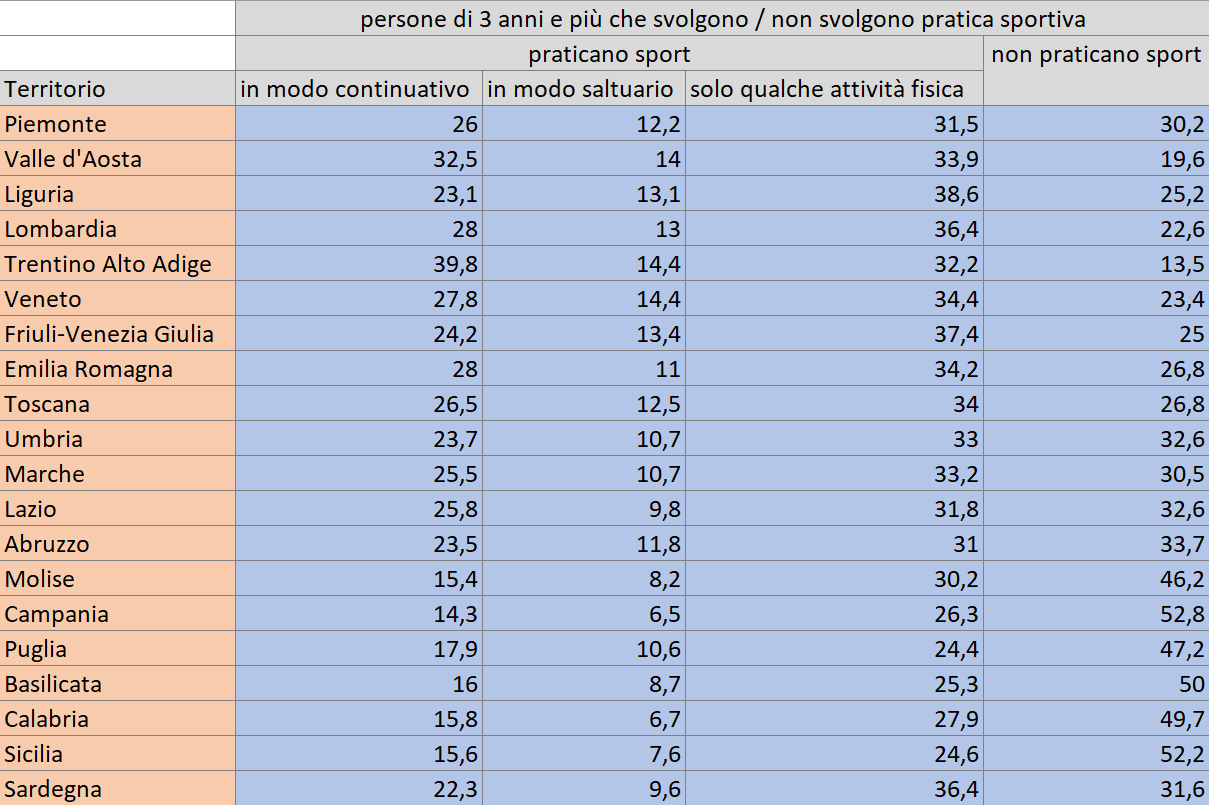
\includegraphics[height=11cm]{ProgettoSAD/capitoli/images/dataset_image.png}
    \caption{Dataset di riferimento.}
    \captionsetup{font={footnotesize,bf,it}}
    \label{fig:dataset_image}
\end{figure}

Al fine di poter lavorare in R sul dataset esportato, esso viene inserito all'interno di un \textbf{dataframe}.

\vspace{5mm}
\begin{lstlisting}
regioni <- c("Piemonte", "ValleD'Aosta", "Liguria", "Lombardia", "TrentinoAltoAdige",
             "Veneto", "Friuli-VeneziaGiulia", "Emilia-Romagna", "Toscana", "Umbria",
             "Marche", "Lazio", "Abruzzo", "Molise", "Campania", "Puglia",
             "Basilicata", "Calabria", "Sicilia", "Sardegna")


df <- data.frame(Modo.Cont. =
                   c(26, 32.5, 23.1, 28, 39.8, 27.8, 24.2, 28, 26.5, 23.7, 25.5,
                     25.8, 23.5, 15.4, 14.3, 17.9, 16, 15.8, 15.6, 22.3),
                 Modo.Salt. =
                   c(12.2, 14, 13.1, 13, 14.4, 14.4, 13.4, 11, 12.5, 10.7,
                     10.7, 9.8, 11.8, 8.2, 6.5, 10.6, 8.7, 6.7, 7.6, 9.6),
                 Qualche.Att. =
                   c(31.5, 33.9, 38.6, 36.4, 32.2, 34.4, 37.4, 34.2, 34, 33,
                     33.2, 31.8, 31, 30.2, 26.3, 24.4, 25.3, 27.9, 24.6, 36.4),
                 Non.Prat.Sport. =
                   c(30.2, 19.6, 25.2, 22.6, 13.5, 23.4, 25, 26.8, 26.8, 32.6,
                     30.5, 32.6, 33.7, 46.2, 52.8, 47.2, 50, 49.7, 52.2, 31.6))
row.names(df) <- regioni
\end{lstlisting}
\vspace{5mm}

Attraverso la funzione \textit{data.frame()} si è organizzato il dataset in righe e 
colonne. In particolare le colonne sono state costituite come vettori di valori 
numerici tramite la funzione di concatenazione \textit{c()}, attribuendo a ciascuna 
colonna il nome della relativa caratteristica. Successivamente le righe del 
dataframe sono state rinominate con i nomi delle regioni italiane attraverso 
la funzione \textit{row.names(dataset)}.



%################################################

\newpage